% !TeIX spellcheck = cs_CZ
%{\tikzset{external/prefix={tikz/FYZII/}}
% \tikzset{external/figure name/.add={ch09_}{}}
%---------------------------------------------------------------------------------------------------
% file fey2ch09.tex
%---------------------------------------------------------------------------------------------------
%=========================== Kapitola: Elektřina v atmosféře =======================================
\setchaptertoc
\chapter{Elektřina v atmosféře}\label{fyz:IIchapIX}

  \section{Gradient elektrického potenciálu v atmosféře}\label{fyz:IIchapIXsecI}
  \section{Elektrické proudy v atmosféře}\label{fyz:IIchapIXsecII}
  \section{Původ atmosférických proudu}\label{fyz:IIchapIXsecIII}
  \section{Bouřky}\label{fyz:IIchapIXsecIV}
  \section{Mechanismus oddělování nábojů}\label{fyz:IIchapIXsecV}
  \section{Blesk}\label{fyz:IIchapIXsecVI}

    \begin{figure}[ht!]
      \centering
      \subcaptionbox{\label{fyz:fig689a}}{\luafigure[0.9]{fyz_fig689a.pdf}}               \newline
      \subcaptionbox{\label{fyz:fig689b}}{\luafigure[0.9]{fyz_fig689b.pdf}}
      \caption{
               (\cite[s.~748]{Feynman02})}
      \label{fyz:fig689}
    \end{figure}

    \begin{figure}[ht!] %\ref{fyz:fig690}
      \centering
      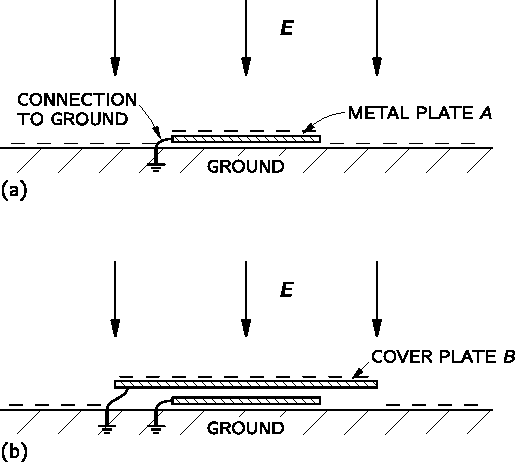
\includegraphics[width=0.6\linewidth]{fyz_fig690.pdf}
      \caption{
               (\cite[s.~707]{Feynman02})}
      \label{fyz:fig690}
    \end{figure}

    \begin{figure}[ht!] %\ref{fyz:fig691}
      \centering
      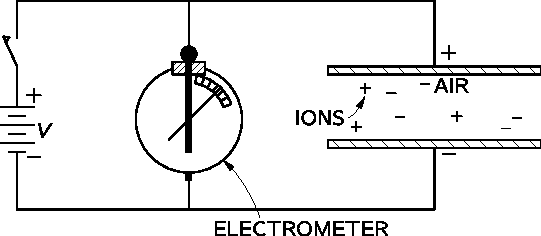
\includegraphics[width=0.6\linewidth]{fyz_fig691.pdf}
      \caption{
               (\cite[s.~707]{Feynman02})}
      \label{fyz:fig691}
    \end{figure}


    \begin{figure}[ht!] %\ref{fyz:fig692}
      \centering
      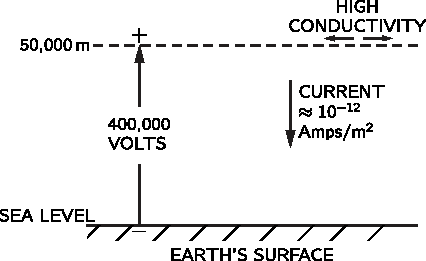
\includegraphics[width=0.6\linewidth]{fyz_fig692.pdf}
      \caption{
               (\cite[s.~707]{Feynman02})}
      \label{fyz:fig692}
    \end{figure}

    \begin{figure}[ht!] %\ref{fyz:fig693}
      \centering
      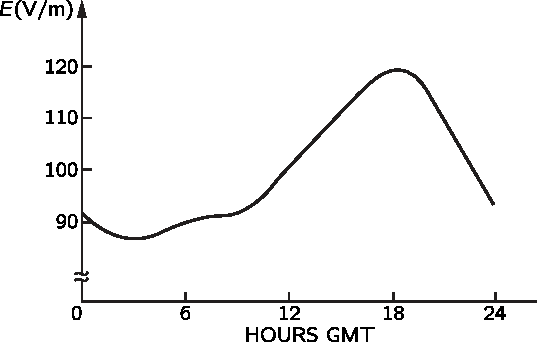
\includegraphics[width=0.6\linewidth]{fyz_fig693.pdf}
      \caption{
               (\cite[s.~707]{Feynman02})}
      \label{fyz:fig693}
    \end{figure}

    \begin{figure}[ht!] %\ref{fyz:fig694}
      \centering
      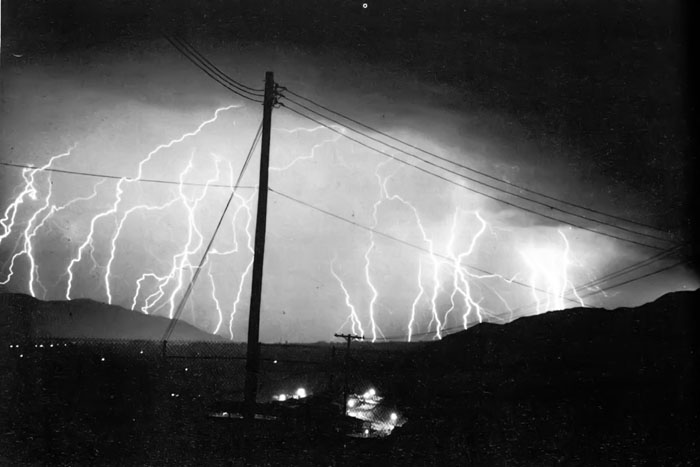
\includegraphics[width=0.6\linewidth]{fyz_fig694.jpg}
      \caption{
               (\cite[s.~707]{Feynman02})}
      \label{fyz:fig694}
    \end{figure}

    \begin{figure}[ht!] %\ref{fyz:fig695}
      \centering
      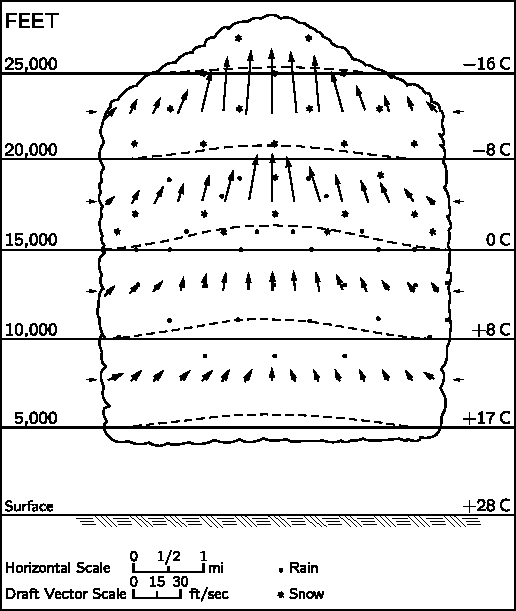
\includegraphics[width=0.6\linewidth]{fyz_fig695.pdf}
      \caption{
               (\cite[s.~707]{Feynman02})}
      \label{fyz:fig695}
    \end{figure}

    \begin{figure}[ht!] %\ref{fyz:fig696}
      \centering
      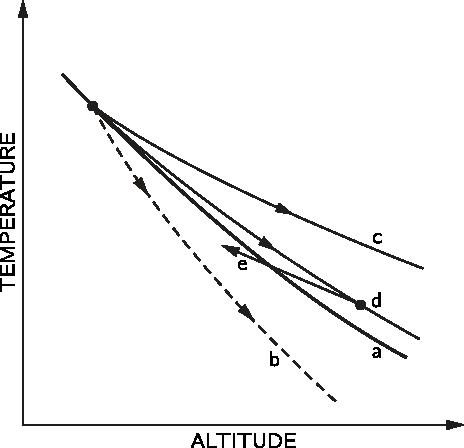
\includegraphics[width=0.6\linewidth]{fyz_fig696.pdf}
      \caption{
               (\cite[s.~707]{Feynman02})}
      \label{fyz:fig696}
    \end{figure}

    \begin{figure}[ht!] %\ref{fyz:fig697}
      \centering
      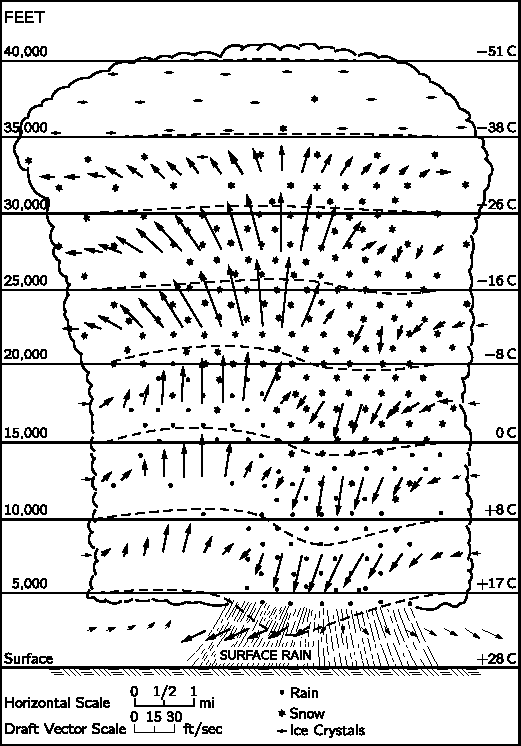
\includegraphics[width=0.6\linewidth]{fyz_fig697.pdf}
      \caption{
               (\cite[s.~707]{Feynman02})}
      \label{fyz:fig697}
    \end{figure}

    \begin{figure}[ht!] %\ref{fyz:fig698}
      \centering
      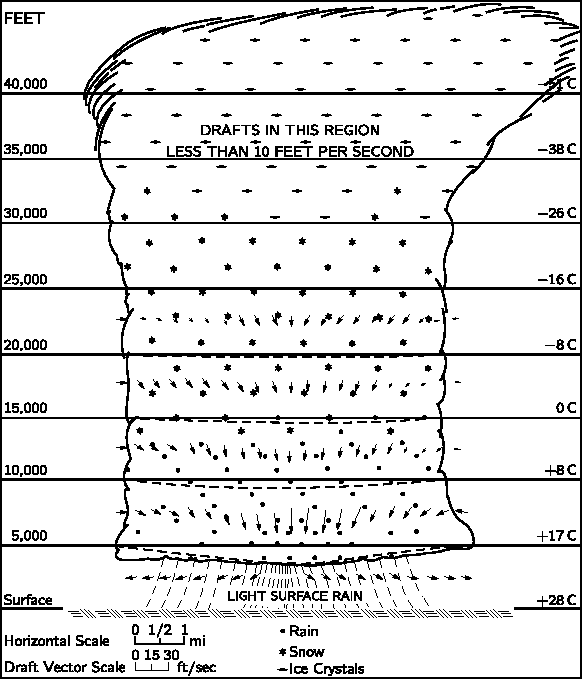
\includegraphics[width=0.6\linewidth]{fyz_fig698.pdf}
      \caption{
               (\cite[s.~707]{Feynman02})}
      \label{fyz:fig698}
    \end{figure}

    \begin{figure}[ht!] %\ref{fyz:fig699}
      \centering
      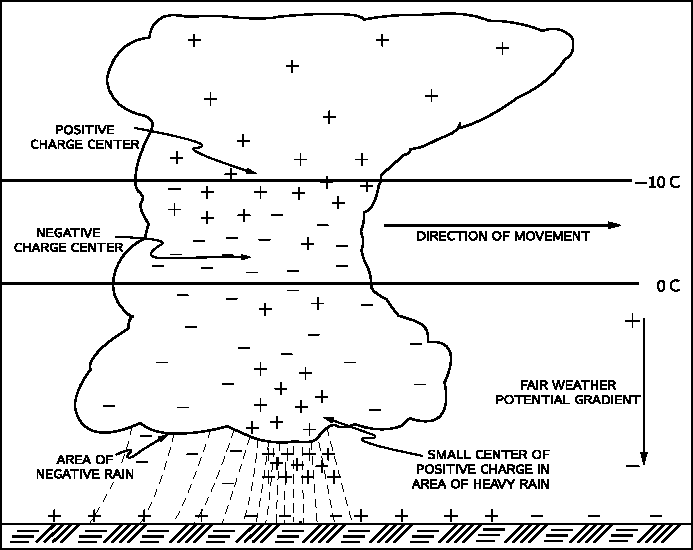
\includegraphics[width=0.6\linewidth]{fyz_fig699.pdf}
      \caption{
               (\cite[s.~707]{Feynman02})}
      \label{fyz:fig699}
    \end{figure}

    \begin{figure}[ht!] %\ref{fyz:fig700}
      \centering
      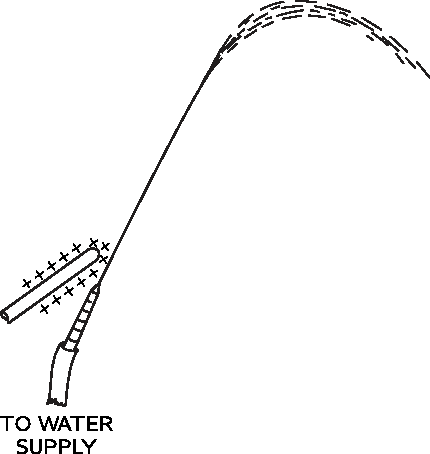
\includegraphics[width=0.6\linewidth]{fyz_fig700.pdf}
      \caption{
               (\cite[s.~707]{Feynman02})}
      \label{fyz:fig700}
    \end{figure}

    \begin{figure}[ht!] %\ref{fyz:fig701}
      \centering
      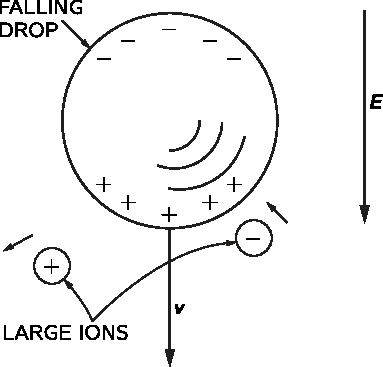
\includegraphics[width=0.6\linewidth]{fyz_fig701.pdf}
      \caption{
               (\cite[s.~707]{Feynman02})}
      \label{fyz:fig701}
    \end{figure}

    \begin{figure}[ht!] %\ref{fyz:fig702}
      \centering
      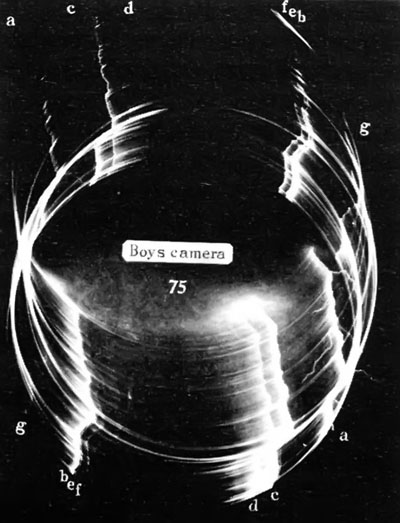
\includegraphics[width=0.6\linewidth]{fyz_fig702.jpg}
      \caption{
               (\cite[s.~707]{Feynman02})}
      \label{fyz:fig702}
    \end{figure}

    \begin{figure}[ht!] %\ref{fyz:fig703}
      \centering
      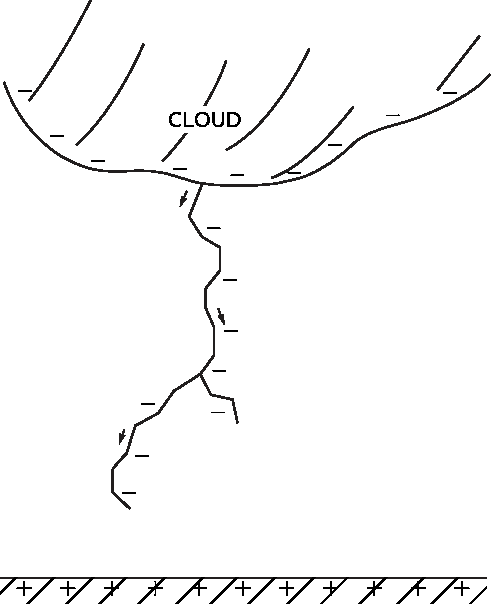
\includegraphics[width=0.6\linewidth]{fyz_fig703.pdf}
      \caption{
               (\cite[s.~707]{Feynman02})}
      \label{fyz:fig703}
    \end{figure}

    \begin{figure}[ht!] %\ref{fyz:fig704}
      \centering
      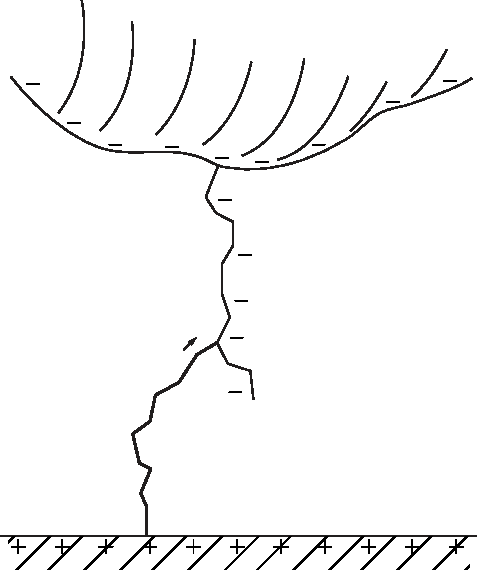
\includegraphics[width=0.6\linewidth]{fyz_fig704.pdf}
      \caption{
               (\cite[s.~707]{Feynman02})}
      \label{fyz:fig704}
    \end{figure}

\todo[inline]{Kapitola fey2ch09 je nedodělaná, obsahuje pouze obrázky}
%} %tikzset
%---------------------------------------------------------------------------------------------------